\documentclass[10pt, oneside]{article}

\usepackage[T1]{fontenc}
\usepackage[utf8]{inputenc}
\usepackage{polski}
\usepackage{indentfirst}
\usepackage{caption}
\usepackage{float}
\usepackage{tikz}
\usepackage{polski}
\usepackage{fancyhdr}
\usepackage{lastpage}
\usepackage{tcolorbox}
\usepackage{graphicx}

\newcommand{\R}[1]{\textcolor{red}{#1}}
\newcommand{\B}[1]{\textcolor{blue}{#1}}
\newcommand{\G}[1]{\textcolor{red}{#1}}

\title{Dokumentacja końcowa projektu "Gra w życie"}
\author{Karolina Czachorska, Katarzyna Stankiewicz}
\date{10 kwietnia 2019 r.}

\pagestyle{fancy}
\fancyhf{} 
\lhead{}
\rhead{} 
	
\rfoot{
\begin{center} Strona \thepage \hspace{1pt} z \pageref{LastPage}
\end{center}
}
%____________________________________________________________________

\begin{document}
\maketitle
\tableofcontents
\newpage	
\section{Ostateczny projekt modułów}

 
\begin{figure}[H]
	\centering
	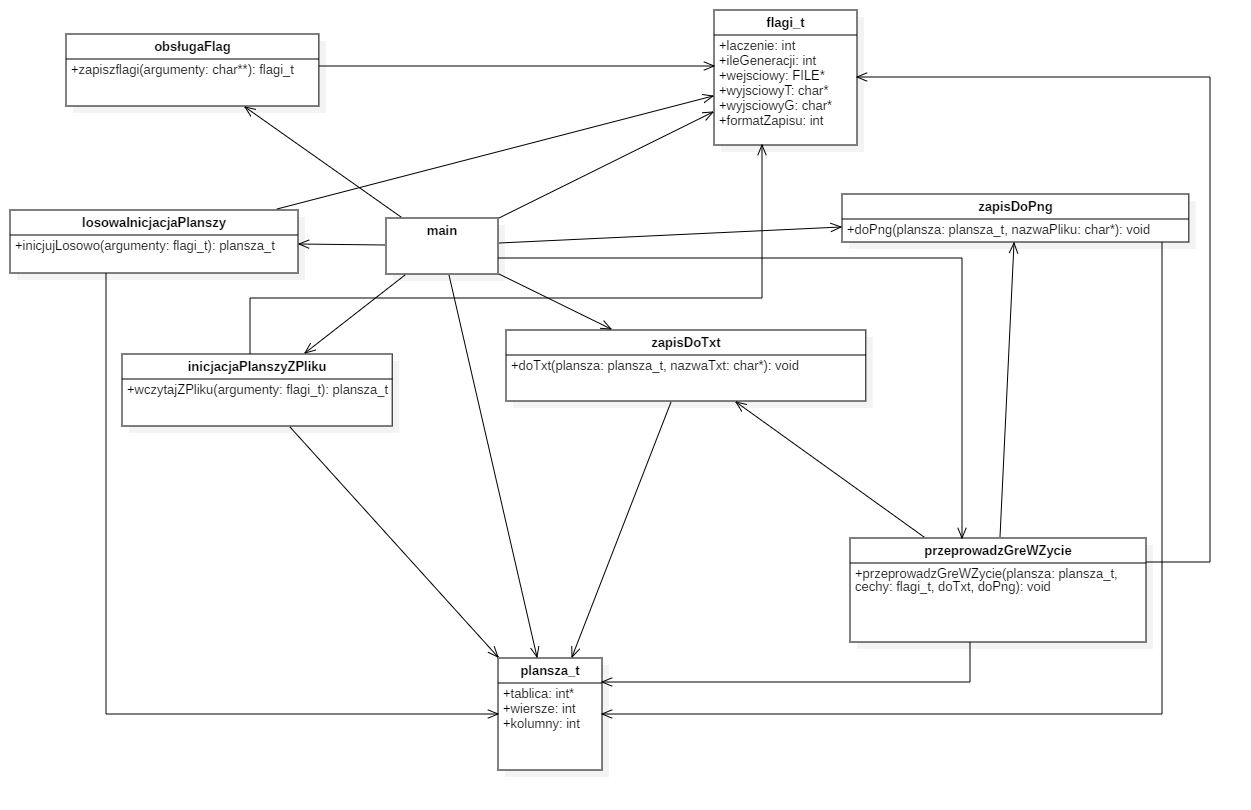
\includegraphics[width=13cm]{Main.png}
\end{figure}

\section{Opis modyfikacji projektu}
Podczas pisania programu zostały przeprowadzone pewne modyfikacje zaplanowanych w początkowej fazie modułów. Zmianom uległy m.in. niektóre nazwy plików. 

\subsection{Moduł przeprowadzGreWZycie}
Moduł generator został zastąpiony nazwą przeprowadzGreWZycie, podobnie funkcja generator znajdująca się w nim, ponieważ jest ona bardziej intuicyjna i lepiej oddaje jego działanie, czyli tworzenie wszystkich generacji planszy oraz zapisywanie ich do plików tekstowych lub graficznych. W module tym została dodana funkcja zapisz, która zajmuje się zapisem do .png oraz .txt. Ma to na celu podział całości na mniejsze funkcje, dzięki czemu kod jest czytelniejszy. 
\subsection{Moduł zapisDoTxt}
Nazwa funkcji doPlikuTxt została zastąpiona przez doTxt. Zmieniona została także kolejność argumentów wywołania funkcji doTxt, tak, aby była analogiczna do kolejności argumentów w doPng. 

\subsection{Moduł obslugaFlag}
Istotną zmianą w module dotyczącym flag jest rezygnacja z możliwości wyboru opcji zawijania kolumn i wierszy. 
Zostały usunięte flagi „łączenie” a dodane „wyświetlanie” umożliwiająca wyświetlenie plansz oraz „pomoc” która wyświetla wskazówki dotyczące wywołania programu. Ponadto zmienione zostały nazwy flag „ileGeneracji” na „generacje” oraz „formatZapisu” na „zapisz”. Na koniec również dodano funkcję zmieniającą typ zmiennej formatZapisu.

\subsection{Struktura plansza t}
Struktura Plansza t została zastąpiona nazwą plansza t, aby ujednolicić schemat nazw modułów, tak aby wszystkie zaczynały się z małej litery. Do plansza t została dodana funkcja wyświetlająca planszę. 

\section{Prezentacja działania}
\subsection{Prawidłowe wywołanie programu}
\subsubsection{Wczytywanie planszy z pliku}
Wywołując program używamy krótkiej wersji flag i podajemy następujące parametry: \\
\begin{itemize}
  \item plik wejściowy: "test.txt"
  \item nazwa pliku do zapisu w formacie .txt: "tekstowy"
  \item nazwa pliku do zapisu w formacie .png: "grafika"
  \item liczba generacji: 14
  \item format zapisu: oba formaty (.png i .txt) 
\end{itemize}
\vspace{15pt}
W rezultacie otrzymujemy następujące wyniki:

\begin{figure}[H]
	\centering
	\includegraphics[width=13cm]{wywolanieProgramu.png}
	\caption{Wywołanie programu z planszą wczytaną z pliku.}
\end{figure}

\noindent Wywołanie programu z powyższymi parametrami spowodowało utworzenie 14 plików o rozszerzeniu ".txt" zawierających kolejne generacje planszy zapisane w formie tekstowej oraz 14 plików o rozszerzeniu ".png" zawierających zapis kolejnych generacji w formie graficznej.

poniżej przedstawiono przykładowe pliki:

\begin{figure}[H]
	\centering
	\includegraphics[width=13cm]{tekstowy.png}
	\caption{wyniki zapisane w formacie tekstowym}
\end{figure}

\begin{figure}[H]
	\centering
	\includegraphics[width=13cm]{graficzny.png}
	\caption{wyniki zapisane w formacie graficznym}
\end{figure}
\subsubsection{Generowanie losowej planszy}
\noindent Wywołując program używamy długiej wersji flag i podajemy następujące parametry: 
\begin{itemize}
  \item rozmiar planszy: 3x3
  \item liczba generacji: 3
  \item format zapisu: png
  \item wyświetlanie: włączone
\end{itemize}

\vspace{15pt} W rezultacie otrzymujemy następujące wyniki:

\begin{figure}[H]
	\centering
	\includegraphics[width=13cm]{wywolanieLosowe.png}
	\caption{Wywołanie programu z wyświetleniem losowo wygenerowanej planszy.}
\end{figure}

W przypadku niepodania pliku z którego ma być wczytana początkowa plansza, jest ona generowana losowo o rozmiarze jaki został podany w argumentach wywołania.
\subsection{Przykładowe błędne wywołania i reakcja programu na błędy}
\noindent Wywołując program używamy flagi zarówno z plikiem zawierającym początkową planszę jak i z rozmiarem, który chcielibyśmy uzyskać w przypadku losowej generacji. 

\begin{figure}[H]
	\centering
	\includegraphics[width=13cm]{plikIrozmiar.png}
	\caption{Wywołanie programu z równoczesnym podaniem nazwy pliku wejściowego i rozmiaru planszy do losowej generacji.}
\end{figure}

Program prawidłowo wczytuje planszę z pliku, ale ignoruje podany rozmiar, wyświetlając komunikat o nieuwzględnieniu parametrów podanych przy fladze dotyczącej rozmiaru. 







\section{Podsumowanie testów modułów}
\subsection{Test modułu zapisDoPng}
Przeprowadzony test zakończył się pomyślnie. \\
Plansza początkowa:\\
\\
0 0 0 1 0 0 0 1 1 1 \\
1 1 1 1 1 0 0 1 0 0 \\
1 1 0 1 1 1 1 0 1 1 \\
0 1 0 0 0 0 0 1 1 0 \\
0 1 1 1 0 0 0 0 1 0 \\
1 0 1 1 0 0 0 1 0 1 \\
1 1 1 1 1 1 1 0 0 0 \\
0 1 1 1 0 0 1 0 0 0 \\
1 1 0 0 1 0 1 1 0 1 \\
1 1 0 0 0 0 1 1 0 0 \\


Plik png:
 


\subsection{Test modułu zapisDoTxt}
Przeprowadzony test zakończył się pomyślnie. \\
\\
Plansza początkowa:\\
0 0 1 0 1 0 0 1 0 0\\
1 0 0 0 0 1 0 1 1 0\\
1 0 0 1 1 0 0 1 0 1\\
0 1 1 0 1 0 0 1 1 0\\
1 0 0 1 1 1 0 1 0 0\\
1 1 0 0 1 1 0 1 0 0\\
0 1 1 1 1 0 1 1 1 0\\
0 1 0 0 0 1 1 1 0 0\\
1 0 1 1 0 0 1 0 1 1\\
0 1 0 0 0 1 0 1 1 0\\
\\
Plansza zapisana do pliku:\\
0 0 1 0 1 0 0 1 0 0\\
1 0 0 0 0 1 0 1 1 0\\
1 0 0 1 1 0 0 1 0 1\\
0 1 1 0 1 0 0 1 1 0\\
1 0 0 1 1 1 0 1 0 0\\
1 1 0 0 1 1 0 1 0 0\\
0 1 1 1 1 0 1 1 1 0\\
0 1 0 0 0 1 1 1 0 0\\
1 0 1 1 0 0 1 0 1 1\\
0 1 0 0 0 1 0 1 1 0\\

\subsection{Test modułu przeprowadzGreWZycie}
Przeprowadzony test zakończył się pomyślnie.\\ 
Kolejne generacje planszy:\\
1 0 1 1 \\
0 1 0 1 \\
0 0 1 1 \\
0 1 1 1 \\
\\
0 1 1 1 \\
0 1 0 0 \\
0 0 0 0 \\
0 1 0 1 \\
\\
0 1 1 0\\ 
0 1 1 0 \\
0 1 0 0 \\
0 0 0 0\\


\subsection{Test modułu inicjacjaPlanszyZPliku}
Przeprowadzony test zakończył się pomyślnie. Program zapisał planszę odczytaną z pliku „test.txt” zawierającego następujące dane:\\
 
\begin{figure}[H]
	\centering
	\includegraphics[width=5cm]{test.png}
\end{figure}

Wypisał je w następujący sposób, zliczając ile plik zawiera kolumn i wierszy:\\

\begin{figure}[H]
	\centering
	\includegraphics[width=13cm]{zPlikuTest.png}
\end{figure}
 

\subsection{Test modułu losowaInicjacjaPlanszy}

W przypadku niepodania pliku wejściowego plansza zostaje wygenerowana losowo\\

\begin{figure}[H]
	\centering
	\includegraphics[width=13cm]{losowaTest.png}
\end{figure}


\subsection{Test modułu obsługi flag}

W przypadku prawidłowego podania wszystkich parametrów program zapisuje je w następujący sposób:\\

\begin{figure}[H]
	\centering
	\includegraphics[width=13cm]{flagiTest.png}
\end{figure}
 
W przypadku podania złych argumentów lub nie podania ich wcale, wyświetla wskazówkę dotyczącą wyświetlenia pomocy.\\

\begin{figure}[H]
	\centering
	\includegraphics[width=13cm]{pomoc.png}
\end{figure}

\end{document}